
\documentclass[a4paper,11pt,onecolumn,final,english,openbib]{scrbook}

% Marges del document
\addtolength{\headheight}{2cm}
%\addtolength{\topmargin}{2cm}
\setlength{\oddsidemargin}{1.0cm}
\setlength{\evensidemargin}{0.5cm}
\setlength{\textwidth}{14.3cm}
\setlength{\parindent}{0mm}

% Paquets
\usepackage[english]{babel}
\usepackage{amsmath, amssymb}
\usepackage[utf8]{inputenc}
\usepackage{listings}  % The main package for code
\usepackage{xcolor}    % Required for syntax highlighting colors
\usepackage{graphicx}
\usepackage{booktabs}
\usepackage{multirow}
\usepackage{pdflscape}
\usepackage{graphicx}
\usepackage{caption}
\usepackage{tabularx}
\usepackage{enumerate,physics}
\usepackage{multirow}
\usepackage{subcaption}  % versión moderna, recomendada
\usepackage{dsfont}
\usepackage{slashed}
\usepackage{textcomp}
\usepackage{url}
\usepackage{hyperref} 
\usepackage{siunitx}
\usepackage{float}
\usepackage{epigraph}
\usepackage[font=small,labelfont=bf]{caption}
\usepackage{tikz}
\usepackage{lineno}
\usepackage{placeins}
%\FloatBarrier
\lstdefinestyle{mypythonstyle}{
    language=Python,
    basicstyle=\ttfamily\small,       % Use a small typewriter font
    keywordstyle=\color{blue},        % Python keywords in blue
    stringstyle=\color{red!60!black},  % Strings in a reddish-black
    commentstyle=\color{green!60!black},% Comments in a dark green
    numbers=left,                   % Show line numbers on the left
    numberstyle=\tiny\color{gray},    % Make line numbers small and gray
    frame=single,                   % Draw a single-line box around the code
    breaklines=true,                % Automatically break long lines
    showstringspaces=false,         % Don't put ugly markers for spaces in strings
    tabsize=4                       % Set tab size
}

% Coses addicionals
\font\afont=cmssbx10 scaled \magstep5     % for the title
\font\bfont=cmssbx10 scaled \magstep4     % for chapter headings
\font\cfont=cmssbx10 scaled \magstep3
\font\dfont=cmssbx10 scaled \magstep2     % for section headings and author name
\font\efont=cmssbx10 scaled \magstephalf

\setcounter{secnumdepth}{3}
\setcounter{tocdepth}{3}
\setlength{\textfloatsep}{10pt}  % space between text and float (table/figure)
\setlength{\floatsep}{10pt}      % space between floats
\setlength{\intextsep}{10pt}     % space between in-text floats and text

\makeatletter
\renewcommand\paragraph{\@startsection{paragraph}{4}{\z@}%
  {-3.25ex\@plus -1ex \@minus -.2ex}%
  {1.5ex \@plus .2ex}%
  {\normalfont\normalsize\bfseries}
}
\makeatother
\renewcommand{\thesection}{\arabic{section}}

\pagestyle{empty}
\pagestyle{headings}

% Document
\begin{document}
\pagenumbering{roman}
\title{Design, Fabrication and Caractherization of  
All-Glass Laser-Written Vapor Cells for Integrated Photonics Applications}
\author{Rubén Piles Delgado}
\maketitle
\tableofcontents
\newpage
\section{Introduction \& Motivation}
Sensors + MEMs + LWVCs + Alkali Gas + Why this technology is better 
\section{Design of Vapor Cells}
\subsection{Initial Considerations \& Constraints}
\subsection{General Design of Individual LWVCs}
\subsection{Wafer-Level Approach}
\subsection{Real Examples}
\section{Fabrication Methods}
\subsection{Initial Considerations \& Constraints}
\subsection{Types of Glasses \& Quality Requirements}
\subsection{Femtolaser Laser}
\subsection{Optical Contact Bonding}
\subsubsection{Introduction}
\subsubsection{Chemical Cleaning \& Activation}
\subsubsection{Plasma-Activated Bonding}
Exposing glass surfaces to plasma ---using a plasma cleaner--- 
has proven to be a crucial step during the pre-bonding 
stage. Plasma (consisting of electrons, ions, free radicals, and 
photons) acts both as a cleaning and an activation agent in 
the context of glass-to-glass bonding and many other applications
\cite{rammhandbook, masteika2014, suniphd}.  
Figure~\ref{fig:plasma_act} illustrates some of the
many different processes that take place on the surface during 
plasma treatment; some of the most relevant ones are:

\begin{figure}[h]
    \centering
    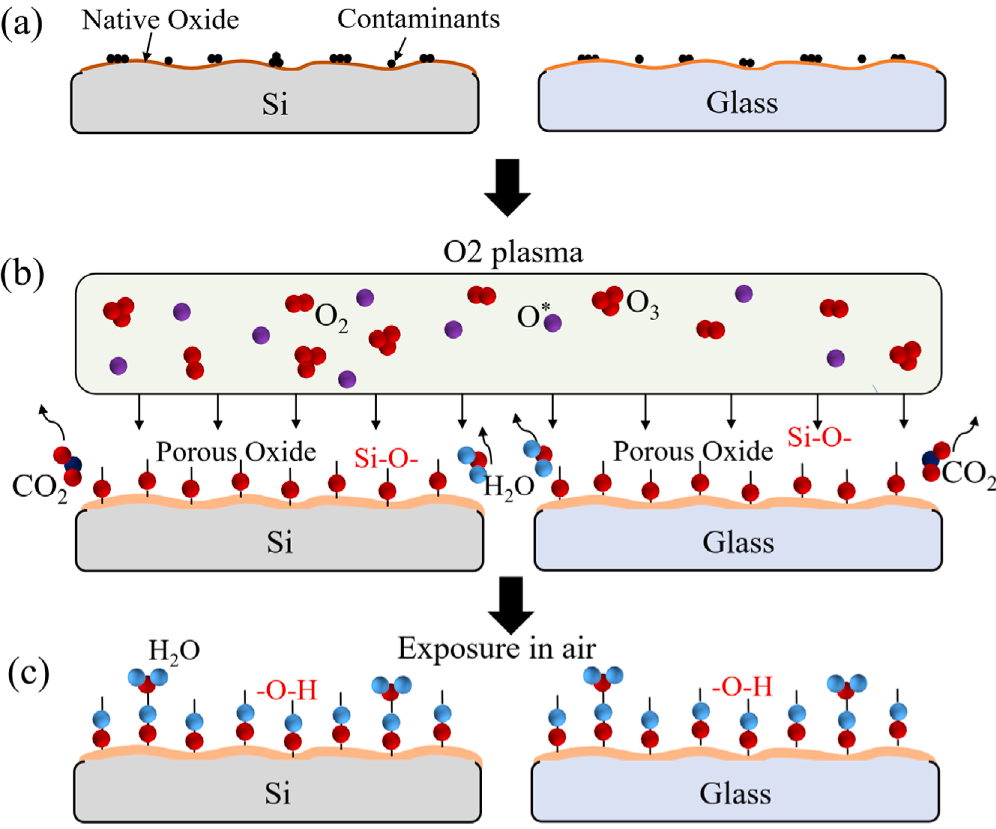
\includegraphics[width=0.75\linewidth]{Images/plasma_activation.png}
    \caption{Effects of plasma treatment on silica surfaces. Plasma helps to remove 
    contaminants while increasing the number of available silanol groups.
    Adapted from \cite{yu2023}}
    \label{fig:plasma_act}
\end{figure}

\begin{enumerate}
    \item \textbf{Removal of contaminants from the surface:} Plasma removes contaminants from
    the surface ---specially organic matter--- and produces more dangling bonds,
    which leads to higher bonded areas.
    \item \textbf{Increase in the number of silanol groups:} 
    Plasma initiates a modification of the surface,
     increasing its number of silanol groups (Si-O-), which are directly correlated to bonding strength.
    \item \textbf{Improvement of the diffusivity of water and gas trapped at the interface:} 
    Plasma treatment increases diffusivity and thus enhances the evacuation of water and gas trapped 
    between the two glass substrates during the bonding stage. 
    Water evacuation is beneficial as it is needed to replace weak, 
    reversible hydrogen bonds ---which play a relevant role to start
    the bonding process--- by stronger Si-O-Si bonds. 
    Removal of trapped gas is also desirable, since it prevents the formation of bubbles during the annealing step.
\end{enumerate}

Common gasses used in these plasma treatments are
 $O_2$, $N_2$, and $Ar$. When operating a plasma cleaner,
 special attention must be paid to its power, chamber pressure, gas flow, and operating 
 times, as overexposure can lead to an increase of surface 
roughness and negatively affect the quality of the final bond.
\\\\
Exposing plasma-treated surfaces to chemicals should be avoided, since these 
substances have the capacity to etch or alter the surface,
effectively eliminating the benefits of this procedure \cite{neumann2021}. Therefore,
plasma treatment should be carried after all chemical cleaning or activation steps.
Nevertheless, exposing plasma-treated surfaces to air or de-ionized water (DIW) has proven to be
beneficial, since water molecules can attach to the Si-O- groups present 
on the surface and create silanol (Si-OH) groups, which are crucial to start the bonding
process between two glass surfaces. Therefore, an effective workflow could be chemical 
cleaning and activation, followed by plasma treatment, a DIW rinse and finally
proceeding with pre-bonding and annealing.
\\\\
Plasma treatment becomes an essential tool in the context of low-temperature optical contact bonding, 
since it can yield 
strong bonding energies even at annealing temperatures as low 
as \SI{100}{\celsius} \cite{eichler2008}.
\subsection{Annealing}
When two sufficiently flat and smooth glass surfaces are brought into contact,
the direct bonding process initiates. One of the first mechanisms to occur is
the formation of hydrogen bonds. These bonds can subsequently be transformed
into stronger covalent bonds, as described by the following chemical reaction:

\begin{equation}
    \mathrm{Si-OH + HO-Si} \rightleftharpoons \mathrm{Si-O-Si + H_2O}.
    \label{eq:polimer siloxane}
\end{equation}
To achieve permanent covalent bonding, water must be removed from the interface,
rendering the aforementioned reaction irreversible \cite{rammhandbook}. This is
accomplished through a thermal treatment known as \textit{annealing}.
\\\\
Annealing involves baking the bonded components in a controlled environment. The
primary parameters influencing the outcome are the temperature ramp, the
equilibrium temperature, and the annealing time. 
\\\\
The \textit{temperature ramp} refers to the heating rate within the oven.
This gradient should be kept as low as possible, as rapid temperature increases
can induce thermal stress in the glass substrates. Such stress may compromise
mechanical and optical performance, or even result in substrate fracture. 
\\\\
Regarding \textit{equilibrium temperatures}, higher values facilitate greater
water diffusivity, thereby removing moisture from the interface more rapidly.
Furthermore, increased viscous flow enhances surface contact \cite{rammhandbook}.
However, high temperatures are often unsuitable for precision optics,
as they may damage optical coatings or integrated electronics \cite{li2013}. 
In such cases, plasma activation is essential, as it increases surface energy
and water diffusivity at significantly lower temperatures \cite{cho2001}. 
This approach is referred to as \textit{Low-Temperature Direct Bonding}.
\\\\
Concerning \textit{annealing times}, literature indicates that bonding energy
increases monotonically over time, whether through a dedicated annealing process
or by leaving surfaces in contact at room temperature. The relationship between
bonding energy and time follows a logarithmic trend:
\begin{equation}
    \gamma \propto \ln\left(\frac{t}{\mu}\right),
\end{equation}
where $t$ is the annealing time and $\mu$ represents a time constant.
The role of annealing is effectively to decrease this $\mu$ constant, 
allowing maximum bonding energy to be
reached much faster. Typical annealing times for optical applications 
range from 2 to 24 hours \cite{cho2001, yu2023, li2013, possl1998,trinh2022}.
An example of how the bonding energy evolves with time can be seen in Figure 
\ref{fig:annealing_time}.
 \begin{figure}[h]
    \centering
    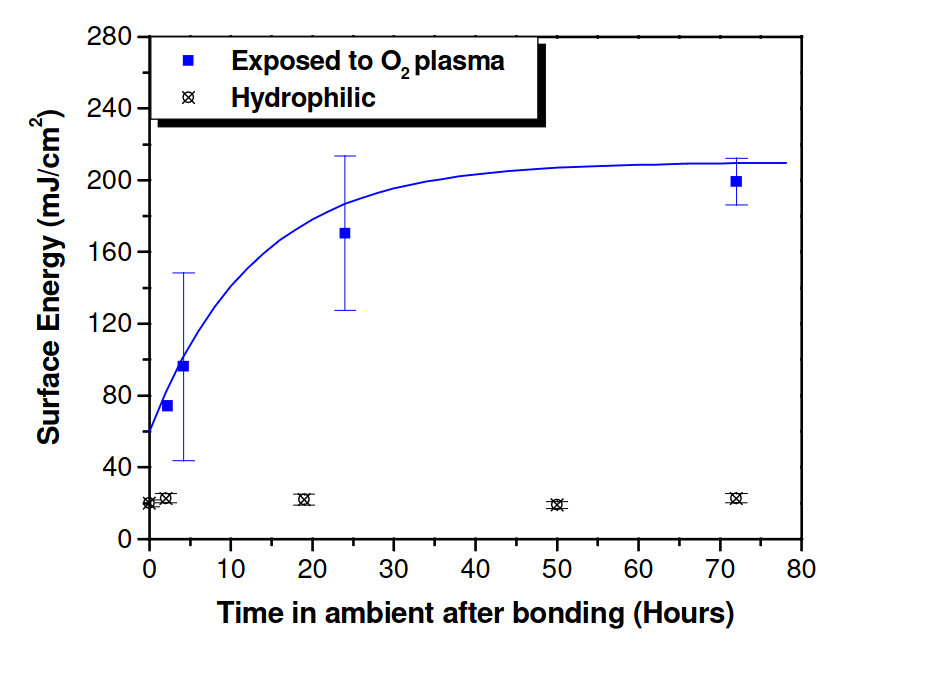
\includegraphics[width=0.8\linewidth]{Images/annealing_time.png}
    \caption{Bonding energy evolution with time. From \cite{cho2001}}
    \label{fig:annealing_time}
\end{figure}   
\subsubsection{Annealing pressure}
In the context of optical contact bonding, mechanical pressure 
applied 
during the annealing phase acts as a vital catalyst by facilitating 
the deformation of surface asperities to increase the degree of intimate
contact \cite{mai2015, trinh2022}, as displayed in Figure \ref{fig:pressure}
    \\\\ This mechanical assistance 
accelerates the kinetics of silanol polymerization, allowing for the 
formation of covalent siloxane bonds at lower temperatures and 
elevating bond energy from typical room-temperature levels 
($<$\SI{0.5}{\joule\per\meter\squared}) to values exceeding 
\SI{2}{\joule\per\meter\squared}, which often surpasses the bulk glass 
fracture toughness \cite{kalk2014}.\\\\ However, pressure must be carefully
optimized; for instance, research on Borofloat 33 wafers indicates 
that a load of \SI{0.07}{\mega\pascal} maximizes flexural strength, 
pressures beyond this limit can lead to stress concentrations and 
premature failure \cite{trinh2022}. Furthermore, non-uniform pressure 
distributions introduce significant risks to device performance, 
such as stress-induced birefringence and permanent wavefront 
distortion \cite{bain2022, wang2014}, necessitating well-planarized 
pressure plates ---with peak-to-valley flatness in the order 
of micrometers--- made of highly stiff materials ---such as technical 
ceramics--- \cite{birckigt2021} for high-precision optical 
and MEMS applications . \\\\
In the setup described by Birckigt et al. \cite{birckigt2021},
pressure is used to enhance contact front propagation during the initial
bonding phase. Convex and concave pressure plates 
---with waviness of \SI{5}{\micro\meter} and 
\SI{3}{\micro\meter},
respectively--- have been employed, as shown in Figure \ref{fig:chucks}.
This setup mitigates the risk of creating interface voids and
introduces radially symmetric residual stresses. 
 \begin{figure}[h]
    \centering
    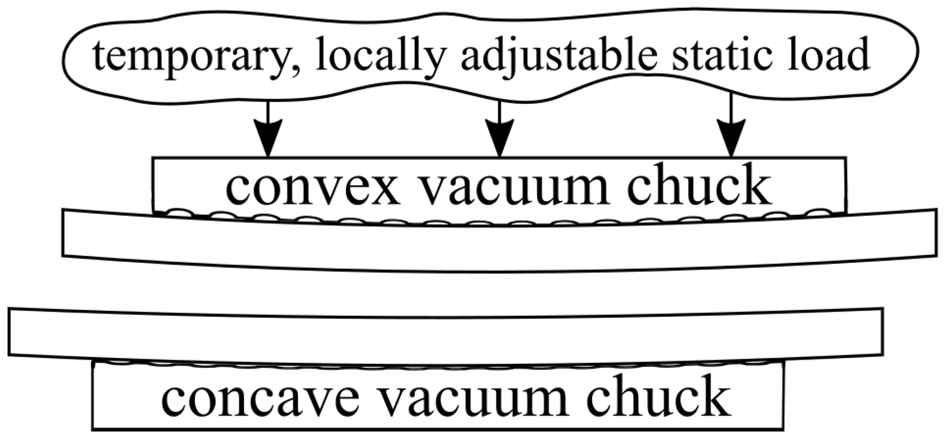
\includegraphics[width=0.8\linewidth]{Images/chucks.png}
    \caption{Setup described by Birckigt et al. \cite{birckigt2021}}
    \label{fig:chucks}
\end{figure}   
\begin{figure}[h]
    \centering
    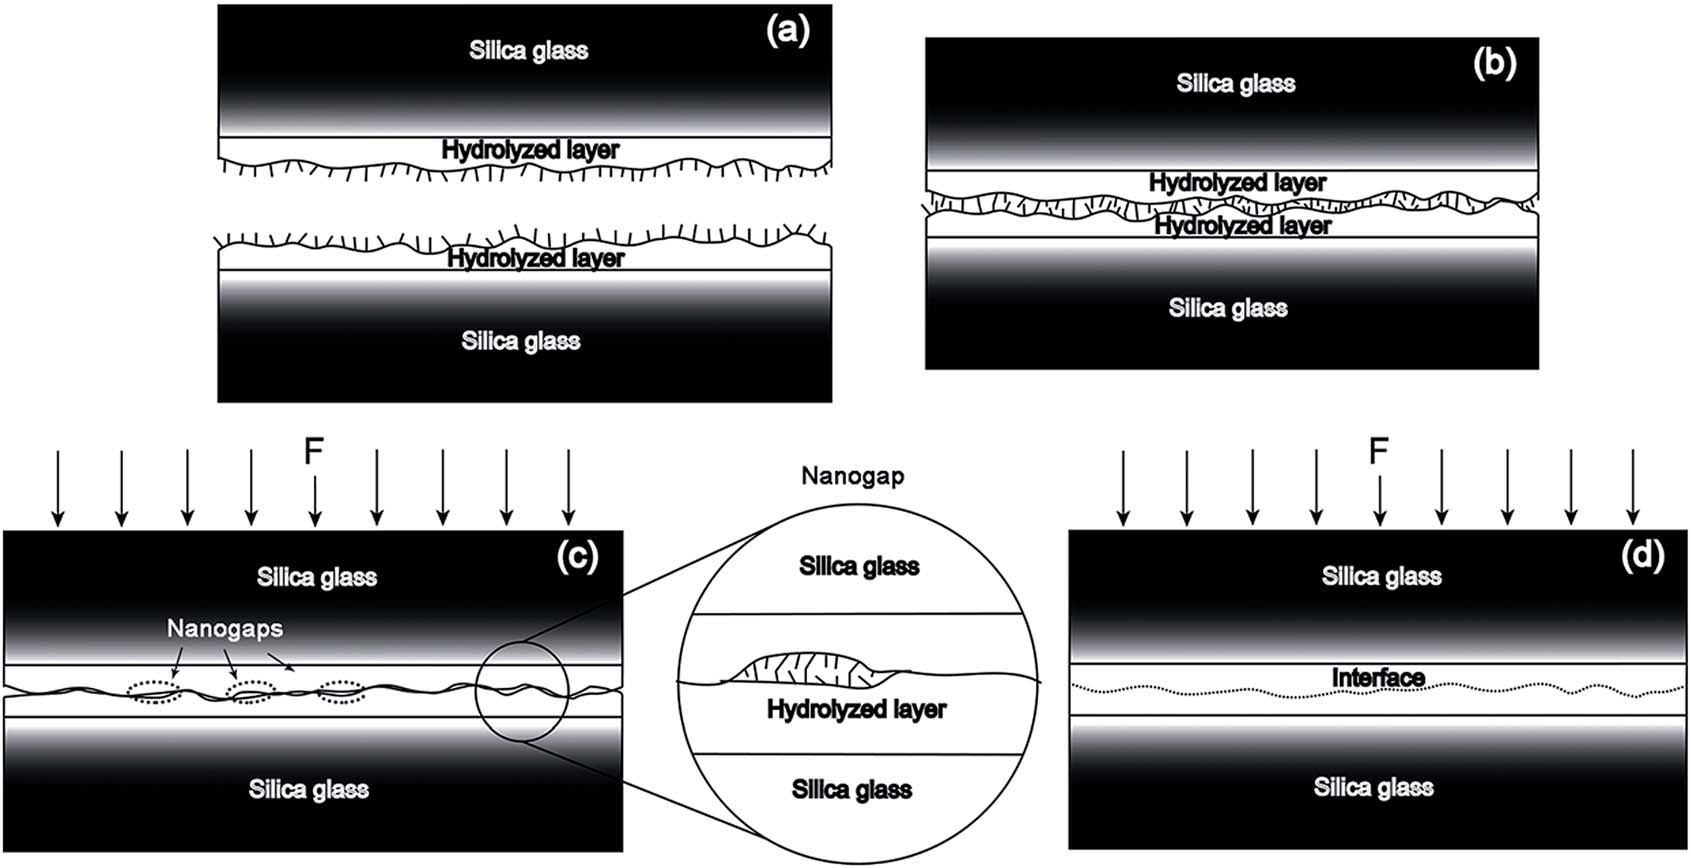
\includegraphics[width=1\linewidth]{Images/pressure.png}
    \caption{Effects of pressure in the bonding process. Interface voids
    can be prevented by applying forces in the direction perpendicular to
    the interface. From \cite{mai2015}}
    \label{fig:pressure}
\end{figure}
\subsection{Other bonding methods}
\subsubsection{Anodic Bonding}
\subsection{Post-Treatments (Coatings, activation)}
\subsection{Step-by-Step Experimental Procedure}
\section{Carachterization and Quality Control}
\subsection{Strength Tests}
\subsection{Surface inspection using an Atomic Force Microscope}
\textit{Atomic Force Microscopy} (AFM) is a sophisticated type of 
scanning probe microscopy, which consists of a physical probe
that scans the specimen in order to produce images of surfaces. 
Atomic Force Microscopes can map the topology of a surface
with sub-nanometric resolution, which makes them an ideal tool 
for surface inspection in the context of atomic sensors, and
more specifically in the context of Optical Contact Bonding,
due to the strict glass roughness requirements of this method. 
\\\\
The AFM consists of a cantilever with a sharp tip at 
its end ---with a radius of curvature 
on the order of nanometers, as shown in \ref{fig:AFM_tip}--- that is used to scan 
the specimen surface. 
When the tip is brought near a sample, forces between them lead to a 
deflection of the cantilever according to Hooke's law. Forces that 
are measured in AFM include mechanical 
contact force, van der Waals forces and capillary forces, among others.
Operating modes are  divided into static \textit{contact} modes and \textit{tapping}
modes, where the cantilever is vibrated at a given frequency.
\begin{figure}[h]
    \centering
    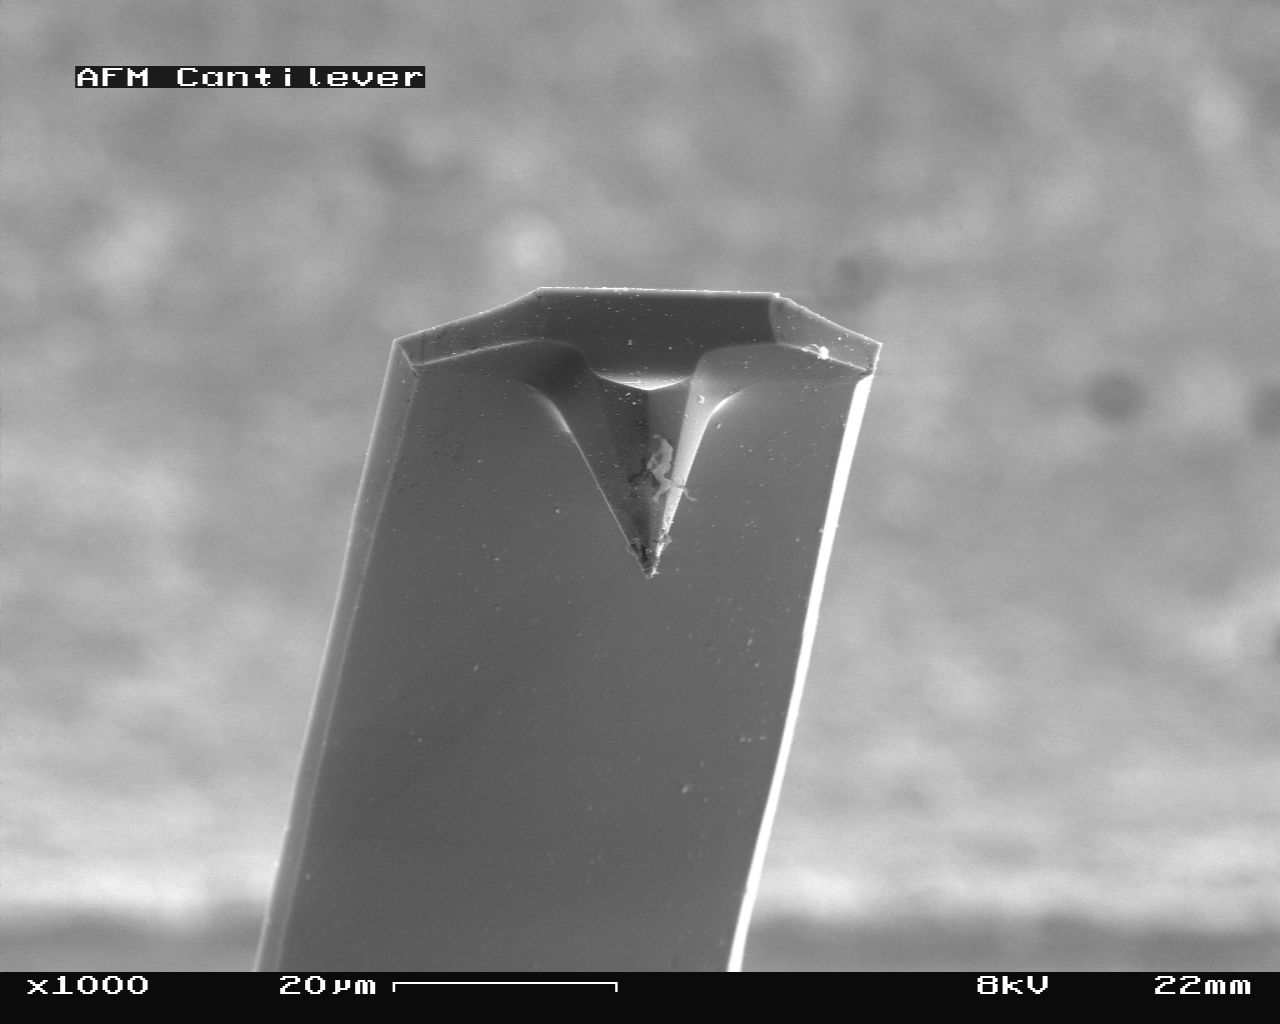
\includegraphics[width=0.6\linewidth]{Images/AFM_tip.JPG}
    \caption{View of cantilever in Atomic Force Microscope (magnification 1000x) \cite{wiki_afm_tip}}
    \label{fig:AFM_tip}
\end{figure}
\\\\
A brand-new Nanoquartz glass disk, with specified Root Mean Square roughness
of \SI{500}{\pico\meter} and Total Thickness Variation (TTV) of \SI{2}{\micro\meter} 
was inspected using a Park NX10 AFM, with a tip Park Scout 350 in \textit{tapping} mode 
(resonance frequency \SI{320}{\kilo\hertz}, rate \SI{0.5}{\hertz}).
It was examined in three different spots of its surface. The obtained data was analyzed
using the \textit{Gwyddion} software, where 
two \ref{fig:AFM_image2D} and three-dimensional \ref{fig:AFM_image3D}
AFM images of the samples were obtained,
along with the density distribution of roughness ---displayed in 
\ref{fig:roughness_dist}. A detailed list of the estimated
surface parameters can be found in \ref{tab:afm}. The precise definition of these parameters 
can be found in \cite{ISO}. 
\begin{figure}
    \centering
    \begin{subfigure}[b]{0.55\textwidth}
        \includegraphics[width=\textwidth]{Images/Sample1_2D_compressed.pdf}
    \end{subfigure}
    \vfill
    \begin{subfigure}[b]{0.48\textwidth}
        \includegraphics[width=\textwidth]{Images/Sample2_2D_compressed.pdf}
    \end{subfigure}
    \begin{subfigure}[b]{0.48\textwidth}
        \includegraphics[width=\textwidth]{Images/Sample3_2D_compressed.pdf}
    \end{subfigure}
    \caption{2D Surface images obtained through AFM in three different
    parts of the pristine Nanoquartz disk's surface.}
    \label{fig:AFM_image2D}
\end{figure}
\begin{figure}
    \centering
    \begin{subfigure}[b]{0.48\textwidth}
        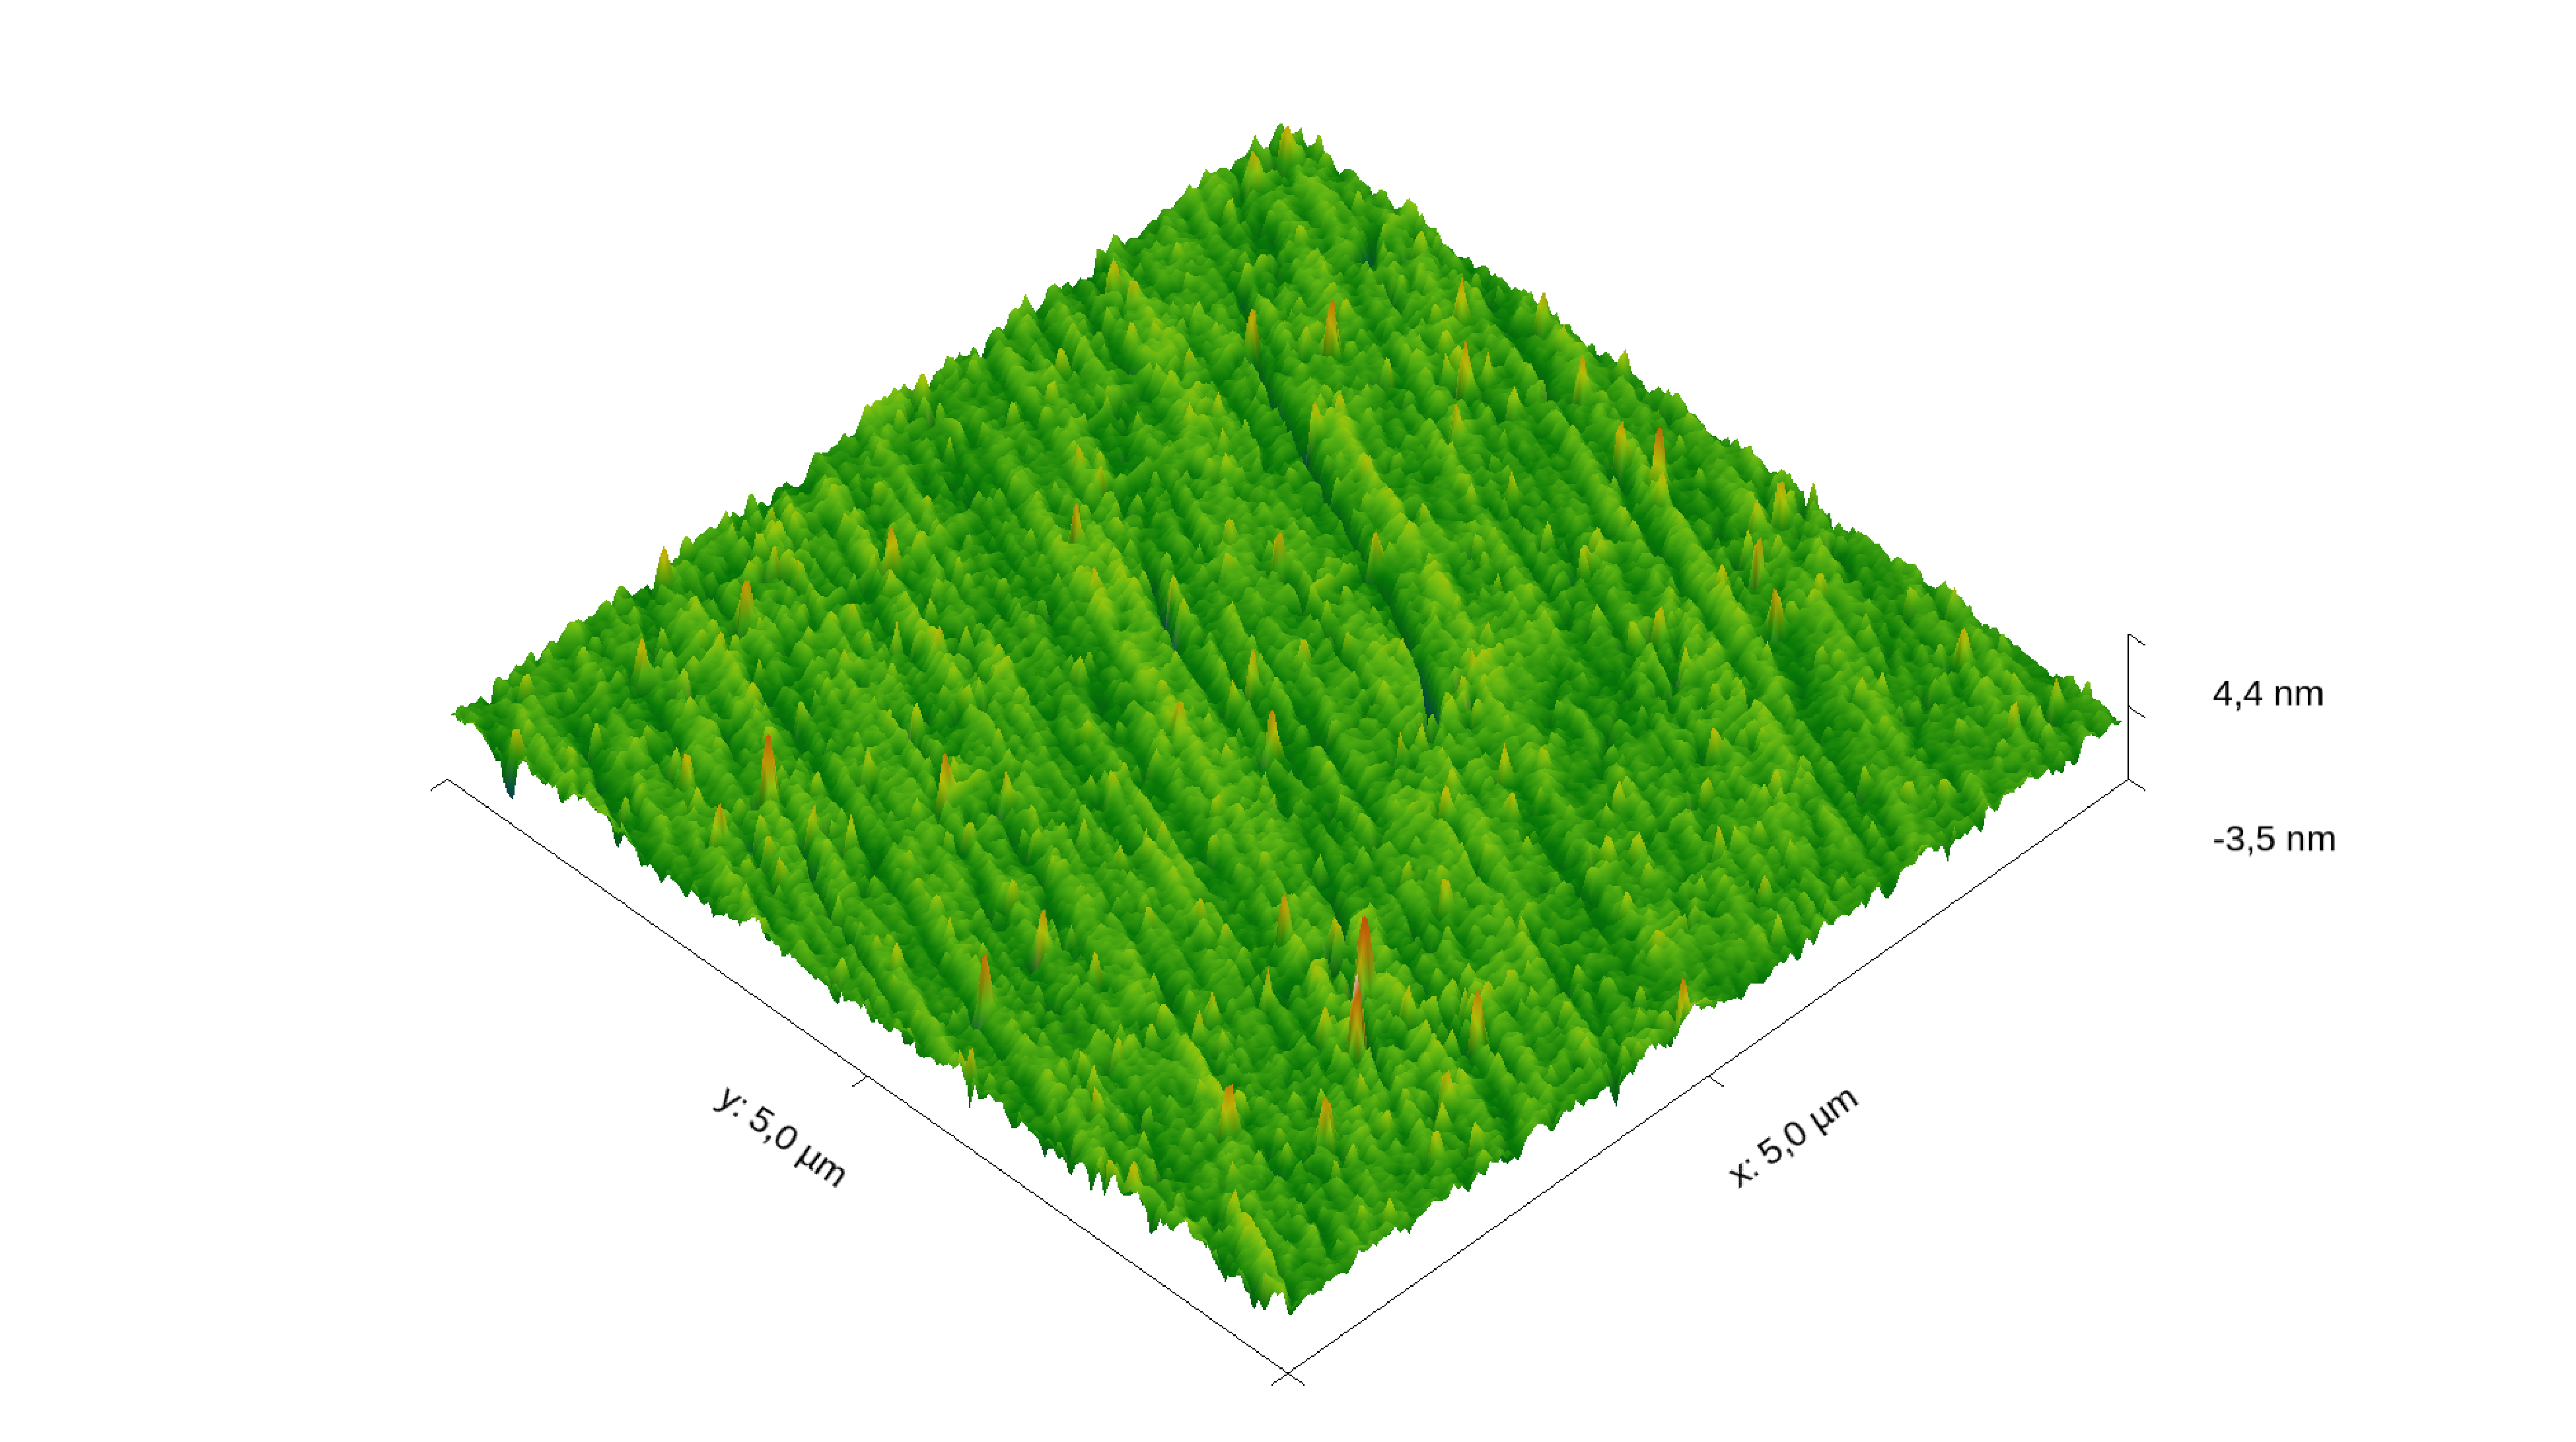
\includegraphics[width=\textwidth]{Images/Sample1_3D.pdf}
    \end{subfigure}
    \vfill
    \begin{subfigure}[b]{0.48\textwidth}
        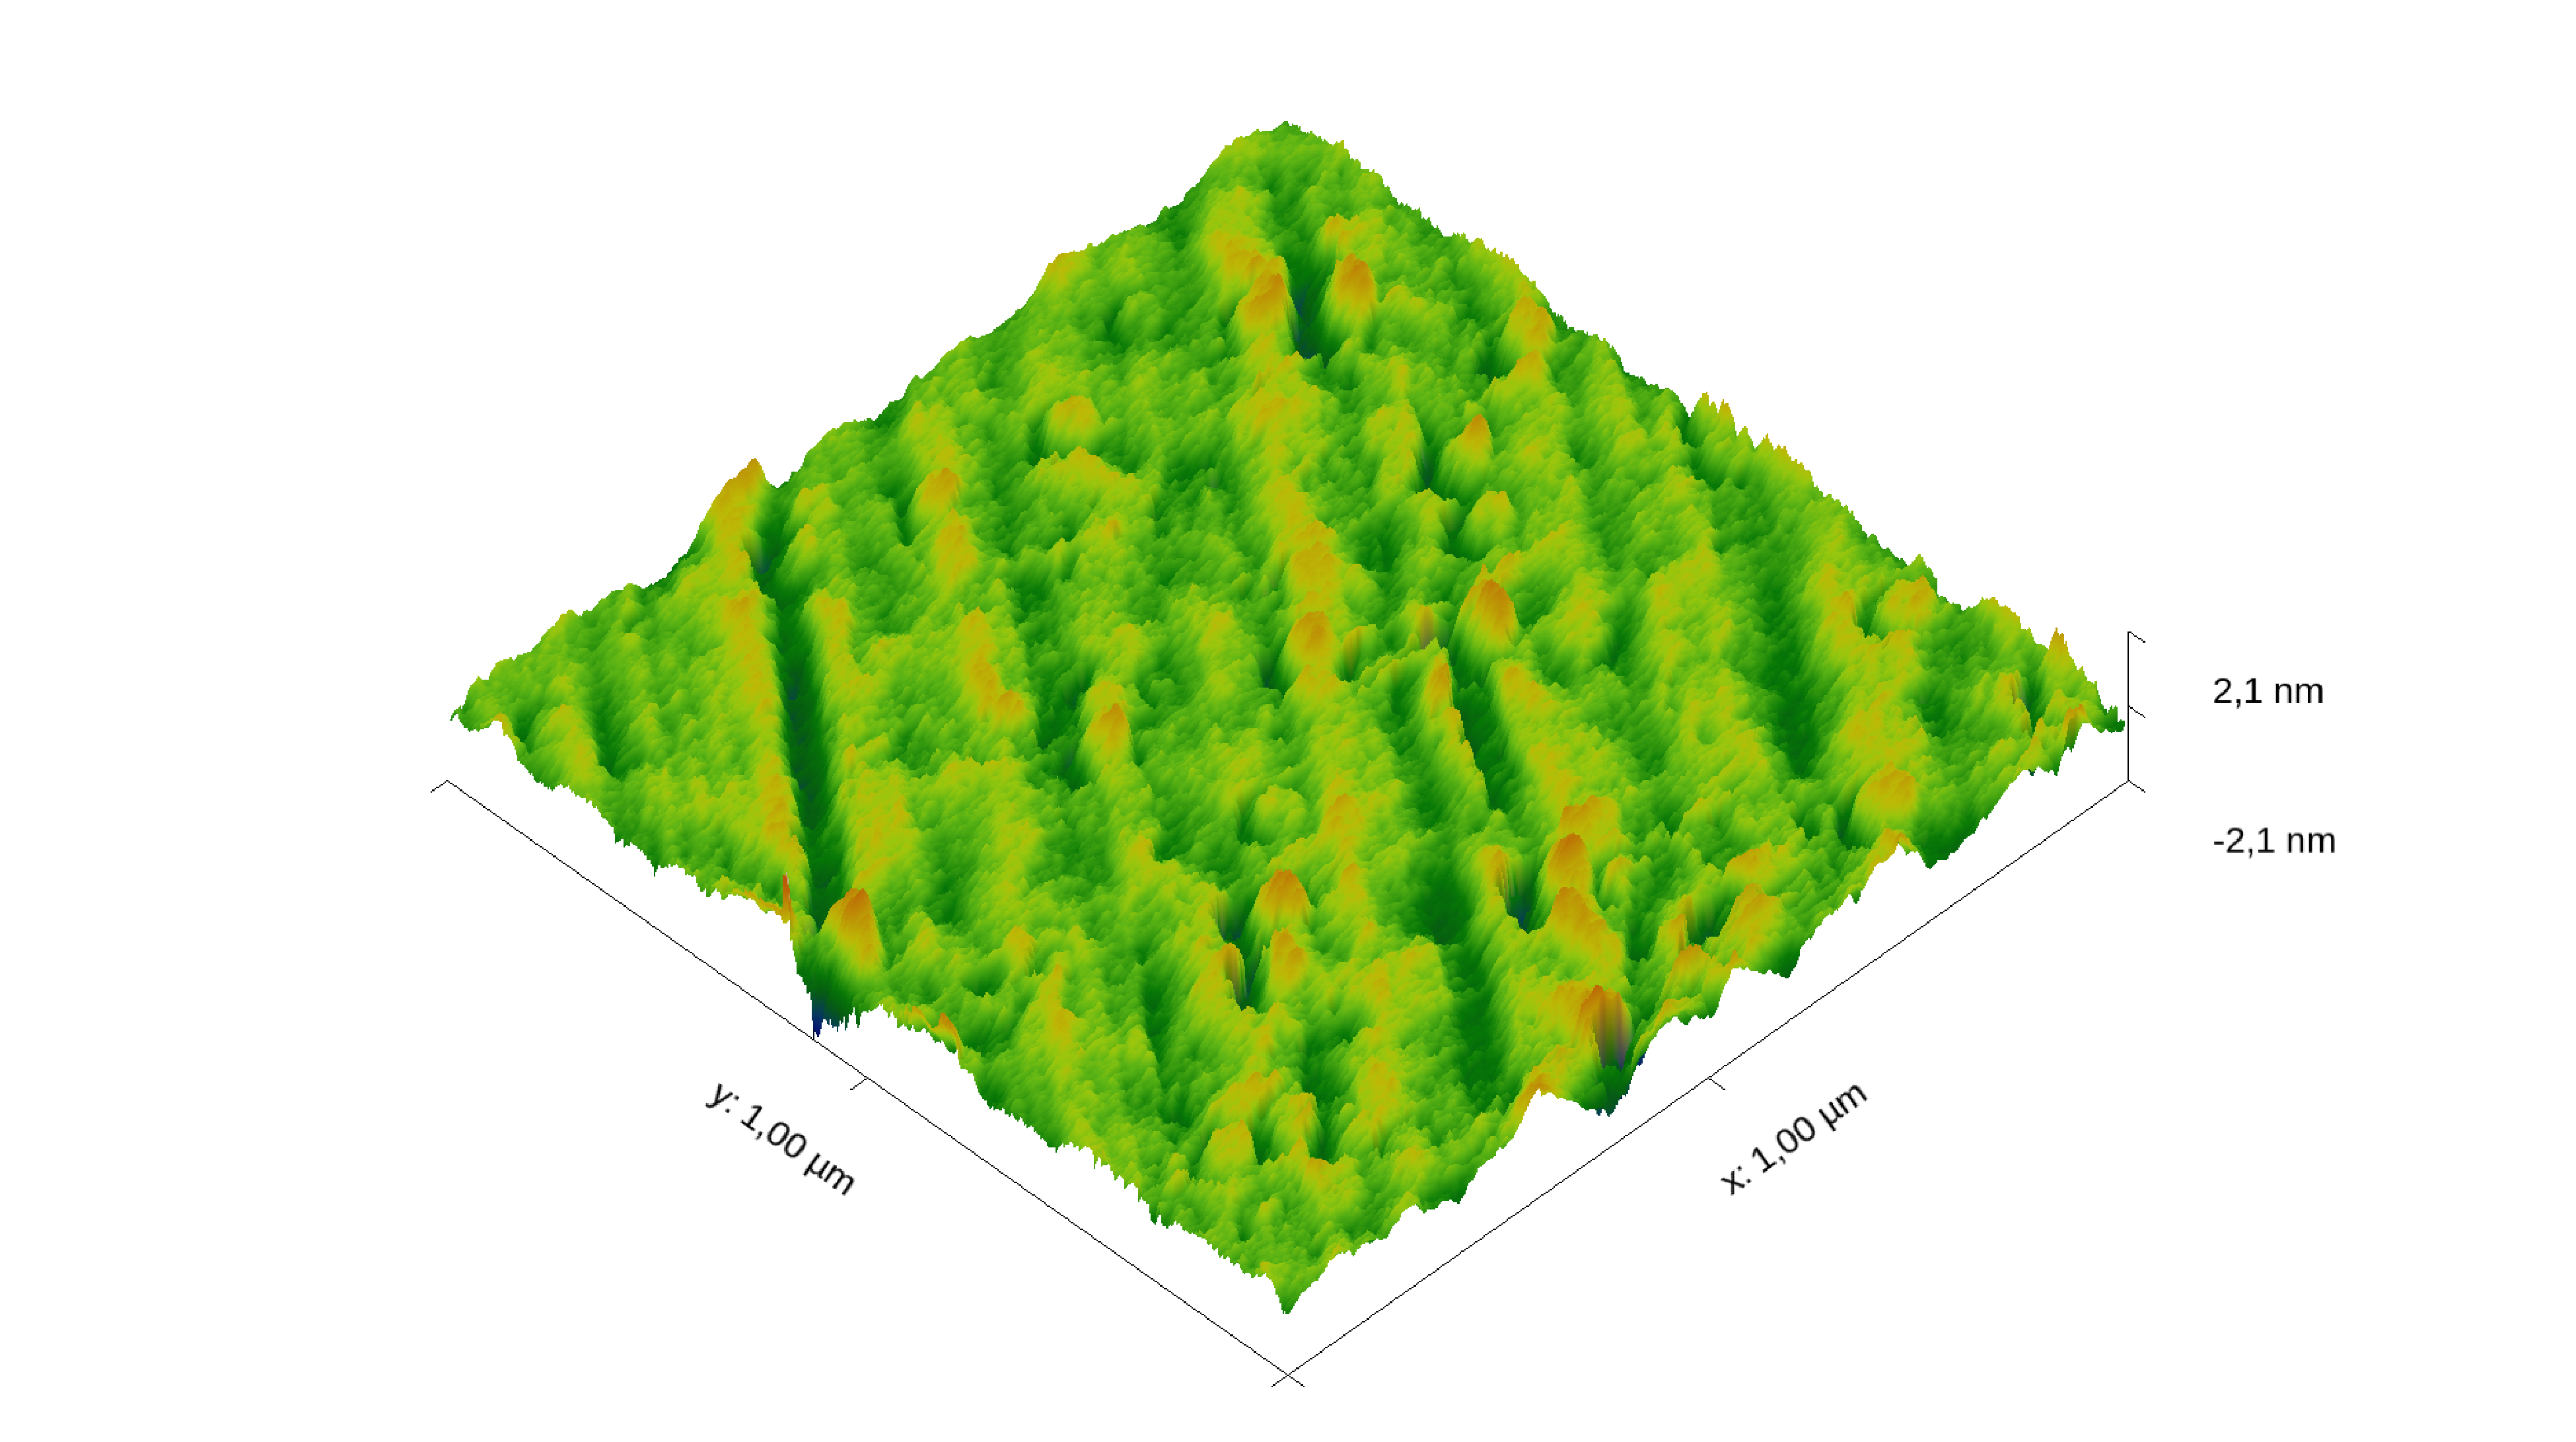
\includegraphics[width=\textwidth]{Images/Sample2_3D.pdf}
    \end{subfigure}
    \begin{subfigure}[b]{0.48\textwidth}
        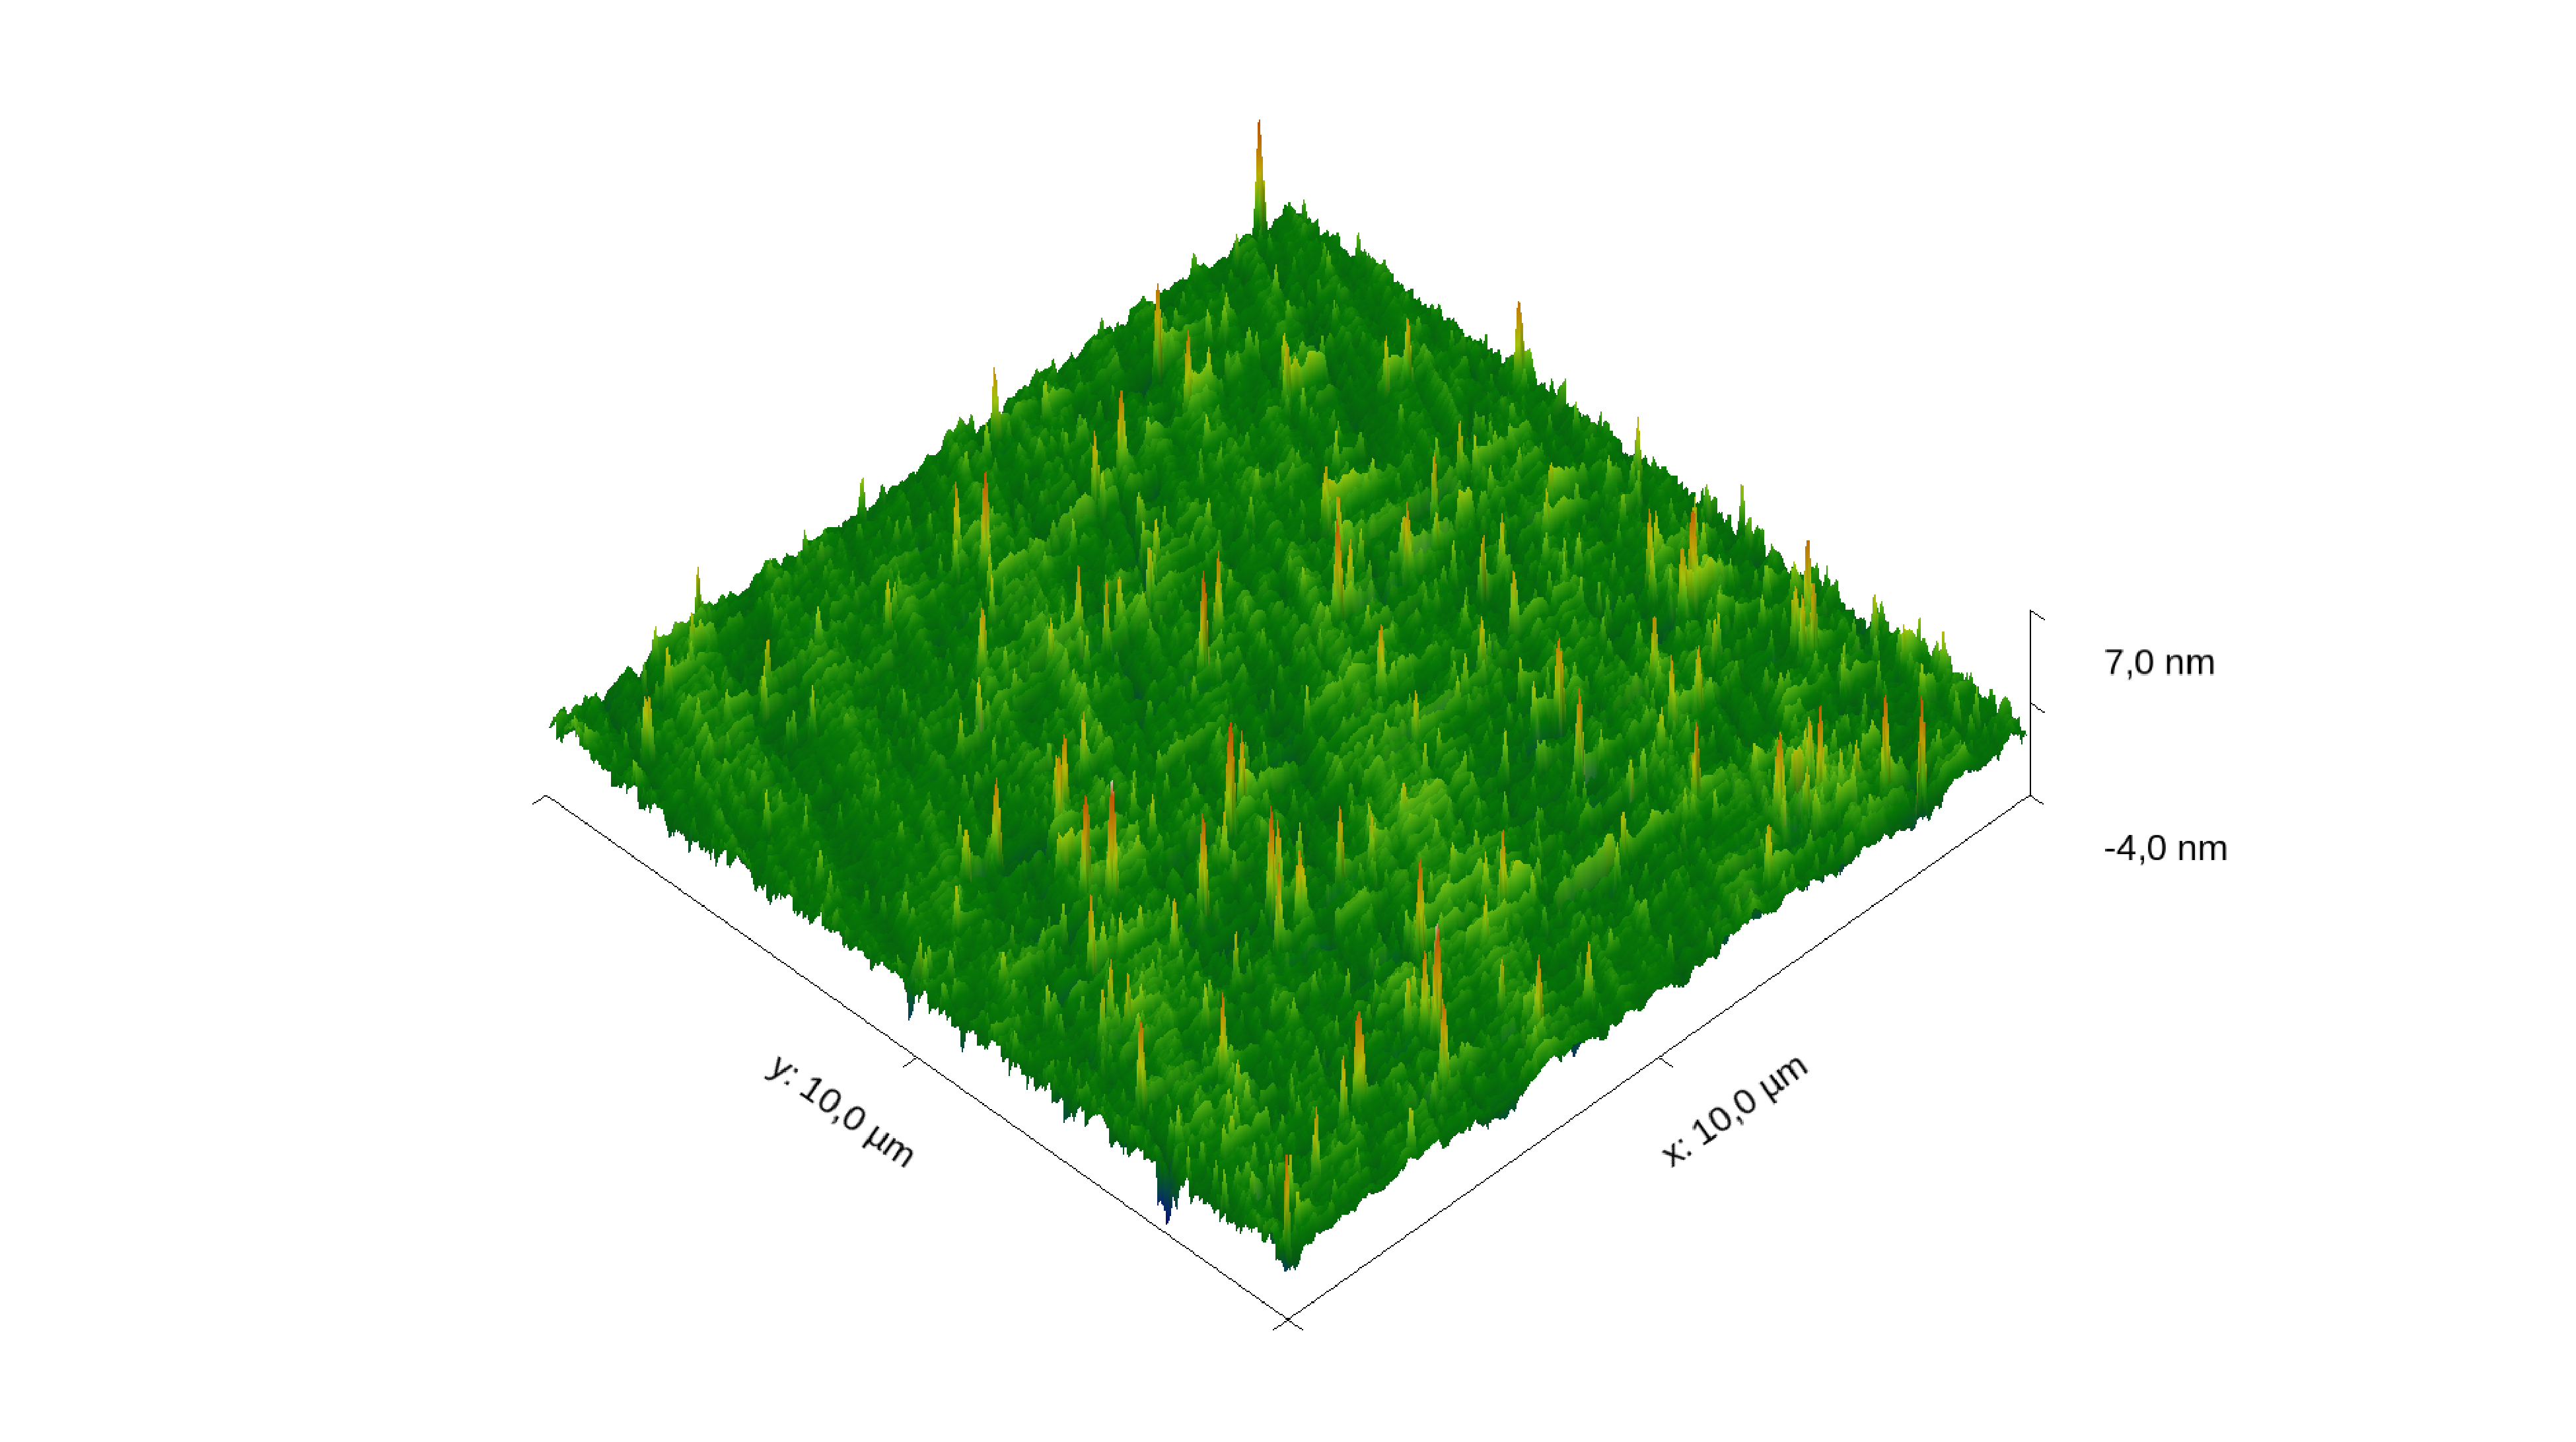
\includegraphics[width=\textwidth]{Images/Sample3_3D.pdf}
    \end{subfigure}
    \caption{3D Surface images obtained through AFM in three different
    parts of the pristine Nanoquartz disk's surface.}
    \label{fig:AFM_image3D}
\end{figure}
\begin{figure}
    \centering
    \begin{subfigure}[b]{0.48\textwidth}
        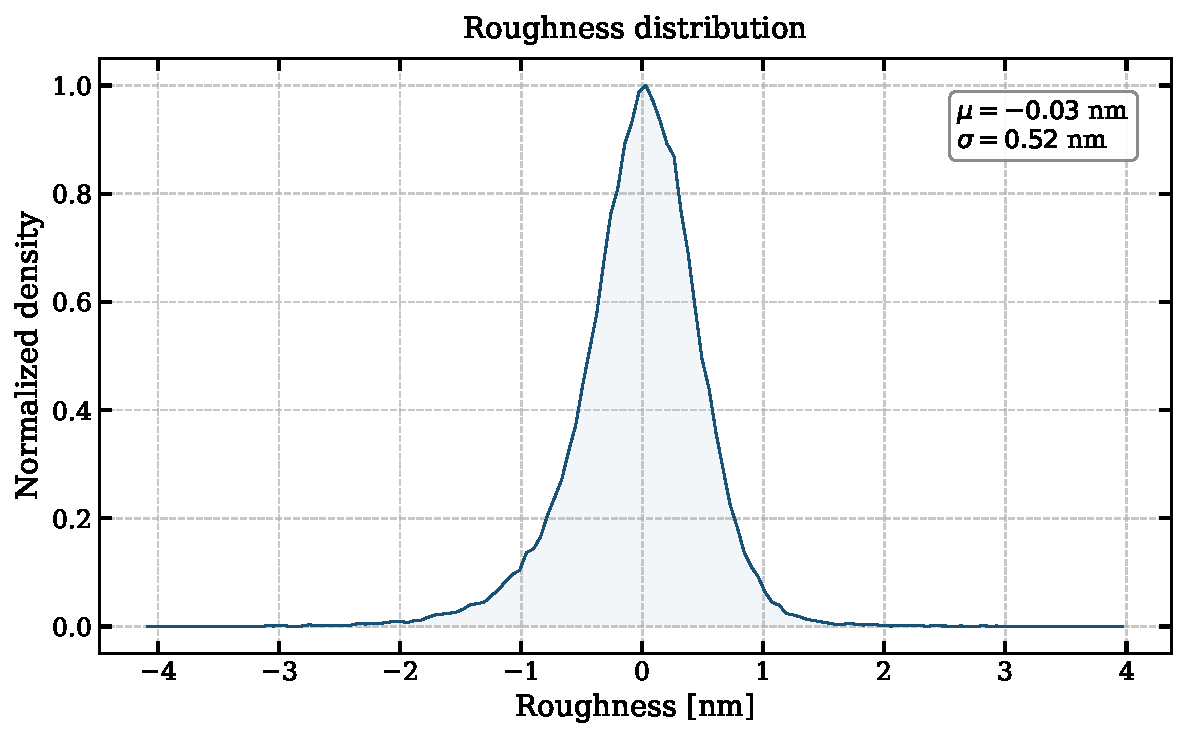
\includegraphics[width=\textwidth]{Images/Sample1_dist.pdf}
    \end{subfigure}
    \vfill
    \begin{subfigure}[b]{0.48\textwidth}
        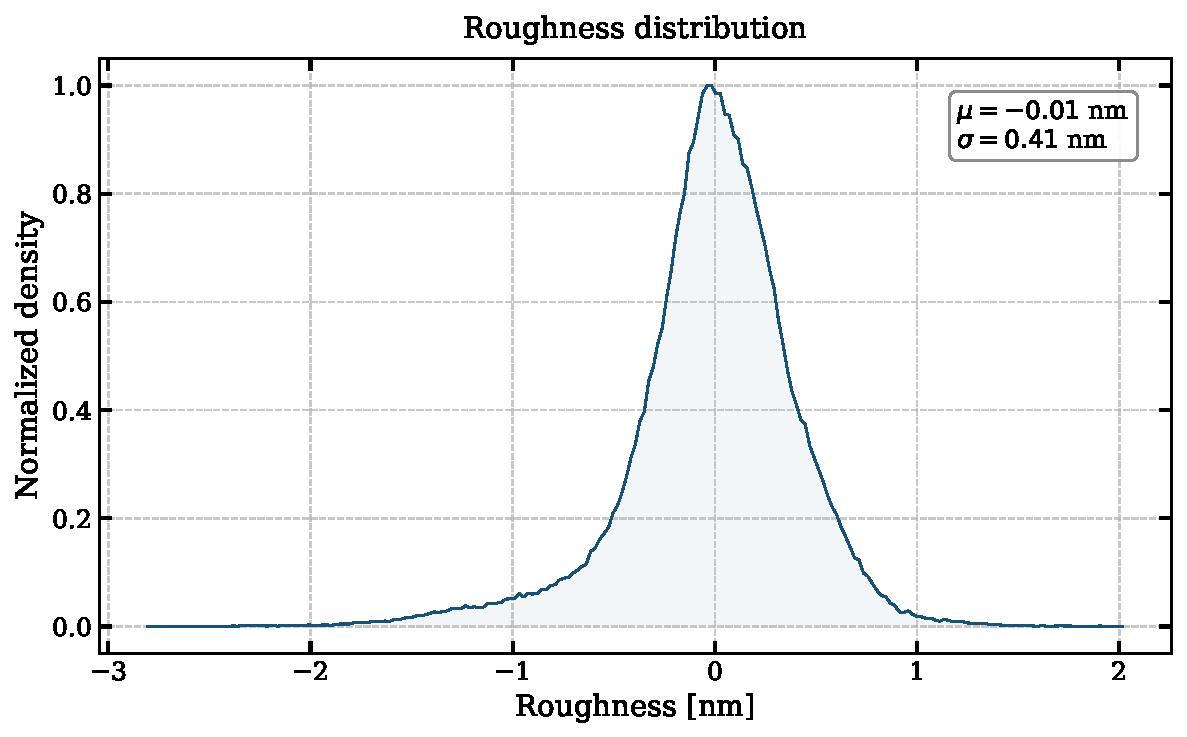
\includegraphics[width=\textwidth]{Images/Sample2_dist.pdf}
    \end{subfigure}
    \begin{subfigure}[b]{0.48\textwidth}
        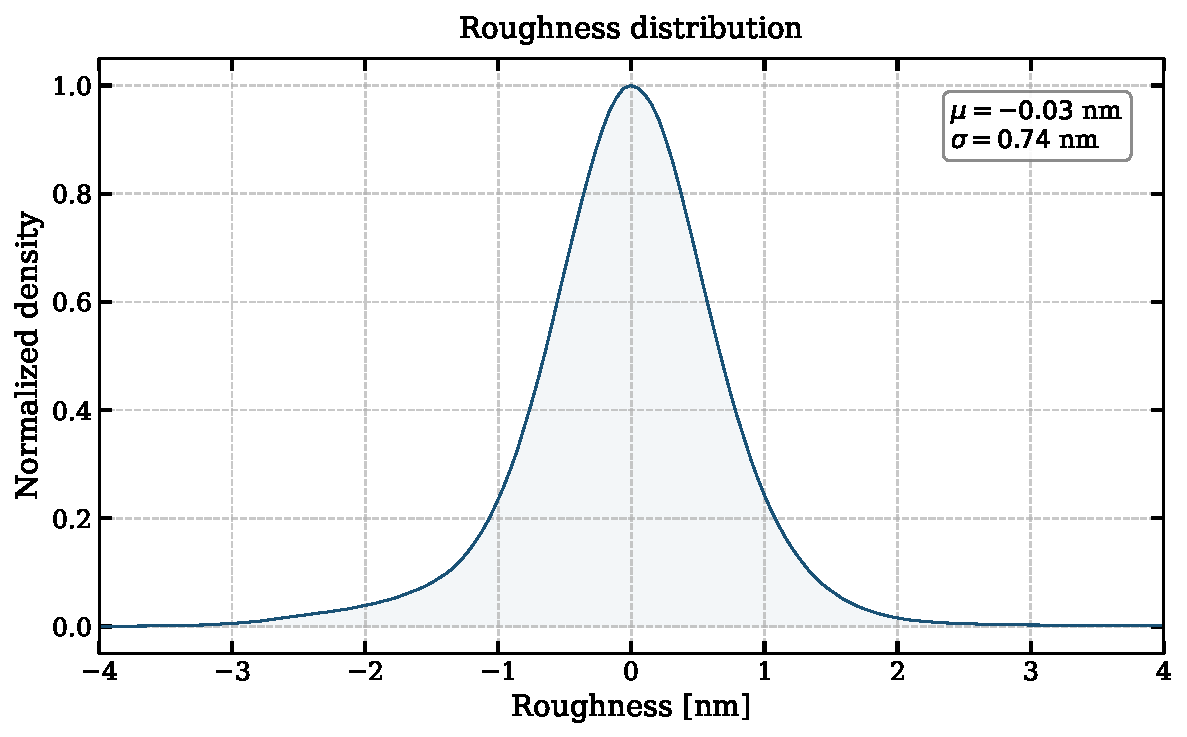
\includegraphics[width=\textwidth]{Images/Sample3_dist.pdf}
    \end{subfigure}
    \caption{Surface roughness distribution obtained through AFM. It can be seen
    that most of the defects are below the \SI{1}{\nano\meter} range. Furthermore,
    the mean ($\mu$) is close to zero, confirming that the surface is uniform.}
    \label{fig:roughness_dist}
\end{figure}
\begin{table}[h]
\centering
\resizebox{\textwidth}{!}{%
\begin{tabular}{l|l|l|l|l|l|l}
\textbf{Sample} & \textbf{$S_q$ {[}pm{]}} & \textbf{$S_a$ {[}pm{]}} & \textbf{$S_p$ {[}nm{]}} & \textbf{$S_v$ {[}nm{]}} & \textbf{$S_z$ {[}nm{]}} & \textbf{Mean height {[}nm{]}} \\ \hline
\textbf{1}      & 518                  & 387                  & 4.02                 & -4.14                & 8.17                 & 0.03                          \\ \hline
\textbf{2}      & 411                  & 298                  & 2.04                 & 2.83                 & 4.87                 & 0.02                          \\ \hline
\textbf{3}      & 726                  & 529                  & 7.66                 & 4.05                 & 11.71                & 0.02                         
\end{tabular}%
}
\caption{Surface parameters obtained through AFM in three different parts of the surface:
\textit{Root mean square roughness} ($S_q$),
 \textit{Mean roughness} ($S_a$), \textit{Maximum peak height} ($S_p$),
 \textit{Minimum valley depth} ($S_v$), \textit{Maximum height} ($S_z$)
 and \textit{Mean height}}
\label{tab:afm}
\end{table}
\\\\
The results confirm that the Root Mean Square roughness of the disk is around \SI{500}{\pico\meter},
as suggested by the manufacturer. An alternative estimation of the surface roughness,
known as \textit{Mean roughness} (Sa) was found to be in the same order of magnitude.
Additionally, it was determined that the total height ($S_q$)
is in the range of a few nanometers. The mean height is approximately zero, 
suggesting that the surface's defects are uniformly distributed. The outstanding surface parameters
observed in this disk comply with Optical Contact Bonding requirements and therefore it is suitable 
for the fabrication of Laser-Written Vapor Cells and high-precission atomic sensors.  
\section{Leak Tests using Spectroscopy}
Once the cell is sealed and activated with the alkali metal 
vapor (typically Rb or Cs), leak tests can be performed over 
time to estimate its hermeticity. Leak tests 
involving laser absorption spectroscopy have been
reported in literature 
\cite{pitz2009, pitz2010, andalkar2002, pitz2014, shi2019}.
 In these tests, a tunable laser 
interacts with the alkali atoms. By measuring the width and 
central frequency of the resulting absorption profile, the 
internal environment of the cell can be monitored.

The optical transitions of alkali metals are characterized 
by the so-called D-line doublet. This fine structure arises
from the spin-orbit interaction, which splits the first
excited state ($nP$) into two distinct energy levels:
$n^2P_{1/2}$ and $n^2P_{3/2}$. The transition from the 
ground state $n^2S_{1/2}$ to the lower excited state
$n^2P_{1/2}$ is known as the D1 line, while the 
transition to the higher state $n^2P_{3/2}$ is the D2 
line. These transitions are illustrated in 
Figure \ref{fig:energy_levels}.
\begin{figure}[h]
    \centering
    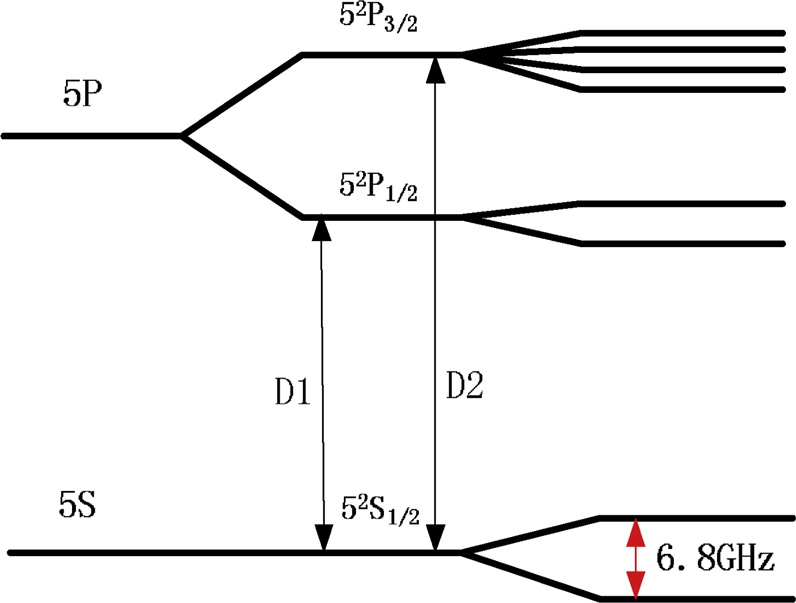
\includegraphics[width=0.5\textwidth]{Images/D1 & D2.png} 
    \caption{Energy level diagram showing the D1 and D2 
    transitions in an alkali metal atom. From \cite{shi2019}}
    \label{fig:energy_levels}
\end{figure}

Collisions between the alkali atoms and other gas molecules
perturb the atomic energy levels, leading to 
collision-induced broadening and a frequency shift. 
If the cell's hermeticity is compromised and atmospheric 
gases leak into the cell, the resulting increase in 
internal pressure ($P$) will cause a detectable width 
broadening and a frequency shift of the Lorentzian profile.
To quantify the gas pressure, the following relations are 
used:
\begin{align}
    \delta \nu &= \delta P \label{eq:delta}
\end{align}
\begin{align}
    \Delta\nu_L &= \gamma P + \gamma_N \label{eq:gamma}
\end{align}

The first equation relates the frequency shift
($\delta\nu$) to the pressure ($P$) through the shift 
rate constant ($\delta$). The second equation links
the pressure to the Lorentzian full width at half maximum
($\Delta \nu_L$), involving the broadening rate constant
$\gamma$ and the natural linewidth $\gamma_N$.

Both $\delta$ and $\gamma$ depend on the specific 
alkali-gas pair and the temperature, with values documented 
in literature 
\cite{pitz2009, pitz2010, andalkar2002, pitz2014, shi2019}.
 Furthermore, the broadening rate $\gamma$ at a temperature
  $T_2$ can be estimated from a known value at $T_1$ using:
\begin{align}
    \gamma(T_2) = \gamma(T_1)\left(\frac{T_1}{T_2}\right)^{\frac{1}{2}}
     \label{eq:gammascale}
\end{align}
Note that the shift constant $\delta$ does not
follow such a simple scaling law due to its more complex 
temperature dependence \cite{pitz2009} 
\subsection{Experimental Proposal}
The spectroscopic framework described above can be directly 
applied to assess the hermeticity of the fabricated vapor 
cells. Here, an experimental procedure similar to the one
followed by Maurice et al.
\cite{maurice2022} is described.

First, the sealed and activated cell is heated to a nominal operating temperature 
$T_\mathrm{op}$ ---chosen so that the alkali vapor pressure 
is sufficient to produce a measurable absorption signal--- 
and held there throughout the measurement campaign using a 
temperature-stabilized mount. Temperature stability is 
critical, since any drift in $T_\mathrm{op}$ would 
introduce a systematic error in the extracted pressure 
through the temperature dependence of $\gamma$ and $\delta$ 
\cite{pitz2009}.

A tunable laser is scanned across the D1 or D2 
absorption line and the transmitted intensity is recorded 
with a photodetector. To avoid power broadening, the probe 
beam intensity is kept well below the saturation intensity 
of the transition. The resulting spectrum is fitted to a 
Voigt profile, from which the Lorentzian width 
$\Delta\nu_L$ and the line center $\nu_0$ are extracted. 
Since the Doppler width depends only on $T_\mathrm{op}$ 
and the atomic mass, the Lorentzian component is 
unambiguously separated. The internal pressure is then 
retrieved using Equations \ref{eq:delta} and \ref{eq:gamma}, evaluated at 
$T_\mathrm{op}$ using literature values of $\gamma$ and 
scaled if necessary via Equation \ref{eq:gammascale}. 
The two estimates of $P$ ---one from the width and one 
from the frequency shift--- serve as a mutual consistency 
check.

Spectra are recorded at regular time intervals: initially 
daily, and subsequently weekly once short-term stability 
has been confirmed. The pressure $P(t)$ is plotted as a 
function of time and, in the case of a small but non-zero 
leak, a linear fit to $P(t)$ yields the leak rate 
$\dot{P}$. If no detectable increase is observed, the 
measurement noise propagated through Equation \ref{eq:gamma} sets 
an upper bound on the leak rate:
\begin{align}
    \sigma_P = \frac{\sigma_{\Delta\nu_L}}
    {\gamma(T_\mathrm{op})}
\end{align}
where $\sigma_{\Delta\nu_L}$ is the uncertainty on the 
fitted Lorentzian width. This bound provides a 
physically meaningful hermeticity statement even in the 
absence of a detectable leak, and allows direct 
comparison with benchmarks from the literature: the 
707-day vacuum integrity demonstrated by 
Artusio-Glimpse et al.~\cite{art2025} using Rydberg 
EIT spectroscopy, and the short-term seal integrity 
inferred from CPT resonance stability by Kobtsev et 
al.~\cite{kobtsev2019} over timescales up to 
$\sim$\SI{1000}{\second}.

\subsection{Enhanced Helium Hermeticity in Micro-fabricated Vapor Cells}
Helium plays a critical role in the operation of various atomic sensors, serving
primarily as a working medium or buffer gas in high-sensitivity applications
(e.g., magnetoencephalography \cite{labyt2019}). However, due to its extremely
small atomic radius, helium exhibits one of the highest permeation rates
through glass walls compared to other gases and alkali metals typically
confined within micro-electromechanical systems (MEMS) vapor cells.
\\\\
For high-precision applications where long-term cell hermeticity is paramount,
aluminum oxide (Al$_{2}$O$_{3}$, or alumina) has been identified as a highly
effective barrier \cite{carle2023, Dellis2016}. Researchers have found that
utilizing aluminosilicate glass---a glass matrix enriched with
Al$_{2}$O$_{3}$---or depositing thin Al$_{2}$O$_{3}$ coatings directly onto
standard glass cells significantly mitigates helium diffusion. 
\\\\
As illustrated in Figure \ref{fig:He}, the permeability constant ($K$) of
aluminosilicate glass is between two and three orders of magnitude lower than
that of conventional borosilicate glass. Furthermore, applying an Al$_{2}$O$_{3}$
coating to borosilicate cells can independently reduce helium permeability by one
to two orders of magnitude. Synergistically combining an aluminosilicate glass
substrate with the aforementioned Al$_{2}$O$_{3}$ coating yields the best results,
achieving ultra-low permeabilities on the order of
$10^{-22}\text{ m}^{2}\text{s}^{-1}\text{Pa}^{-1}$.
\begin{figure}[h]
    \centering
    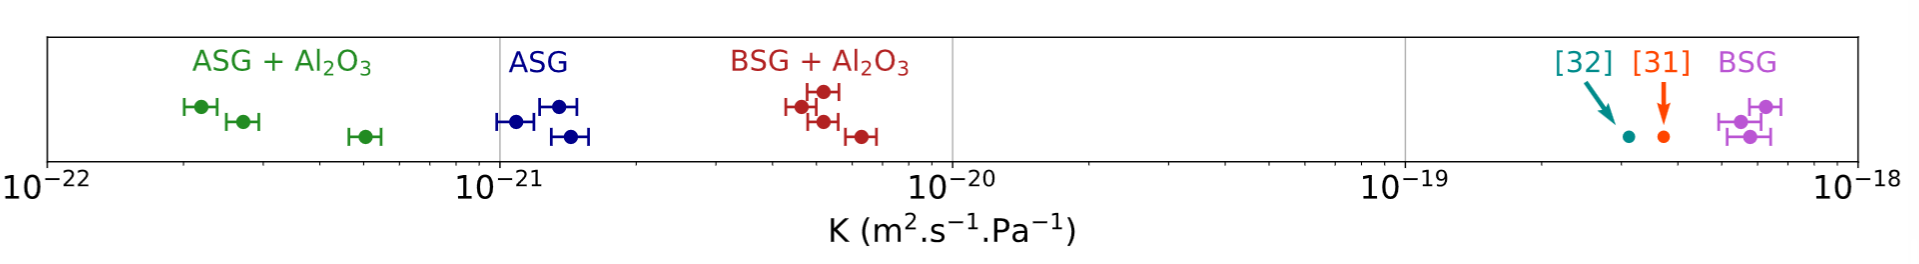
\includegraphics[width=\textwidth]{Images/He.png} 
    \caption{Comparison of the permeability constant $K$ across uncoated borofloat,
     uncoated aluminosilicate, Al$_{2}$O$_{3}$-coated borofloat, and Al$_{2}$O$_{3}$-coated
      aluminosilicate glasses. From \cite{carle2023}.}
    \label{fig:He}
\end{figure}

\section{Experiments \& Applications}
Experiments + magnetometry + space applications + clocks + integration + future applications
\section{Overlook \& Conclusions}
\section{Appendix}
\subsection{Recipes in literature}
\begin{landscape}
\begin{table}[p]
\centering
\caption{Summary of chemical cleaning procedures, surface activation methods, and resulting bonding qualities.}
\label{tab:bonding_procedures_expanded}
\renewcommand{\arraystretch}{1.2} % Da un poco de espacio vertical a las filas
\resizebox{\linewidth}{!}{%
\begin{tabular}{l l l l l l l l l l l}
\toprule
\multirow{2}{*}{\textbf{Reference}} & \multicolumn{7}{c}{\textbf{Chemical Cleaning Steps}} &
 \multirow{2}{*}{\textbf{Surface Activation}} & \multirow{2}{*}{\textbf{Post-Treatment}} & \multirow{2}{*}{\textbf{Bonding Strength}} \\
\cmidrule(lr){2-8}
& \textbf{1} & \textbf{2} & \textbf{3} & \textbf{4} & \textbf{5} & \textbf{6} & \textbf{7} & & & \\
\midrule

Domenico Tuli Thesis 
    & DIW 10' 25$^\circ$C & --- & --- & --- & --- & --- & --- & --- & --- & 0.06 J/m$^2$ \\
    & Acetone 10' 25$^\circ$C & --- & --- & --- & --- & --- & --- & Plasma 30s 15W 35mTorr & --- & 0.06 J/m$^2$ \\
    & Acetone 10' 25$^\circ$C & DIW 10' 25$^\circ$C & Micro Soap 10' 25$^\circ$C & DIW 10' 25$^\circ$C & --- & --- & --- & --- & --- & 0.06 J/m$^2$ \\
    & Acetone 10' 25$^\circ$C & DIW 10' 25$^\circ$C & RCA1 10' 60$^\circ$C & DIW 10' 25$^\circ$C & --- & --- & --- & --- & --- & 0.06 J/m$^2$ \\
    & Acetone 10' 25$^\circ$C & DIW 10' 25$^\circ$C & RCA1 10' 60$^\circ$C & NH$_4$OH 2' 25$^\circ$C & --- & --- & --- & --- & --- & 0.06 J/m$^2$ \\
    & Acetone 10' 25$^\circ$C & DIW 10' 25$^\circ$C & Micro Soap 10' 25$^\circ$C & RCA1 10' 60$^\circ$C & DIW 10' 25$^\circ$C & --- & --- & --- & --- & 0.06 J/m$^2$ \\
    & Acetone 10' 25$^\circ$C & DIW 10' 25$^\circ$C & Micro Soap 10' 25$^\circ$C & RCA1 10' 60$^\circ$C & DIW 10' 25$^\circ$C & --- & --- & --- & --- & 0.1 J/m$^2$ \\
    & Acetone 10' 25$^\circ$C & DIW 10' 25$^\circ$C & Micro Soap 10' 25$^\circ$C & RCA1 10' 60$^\circ$C & NH$_4$OH 2' 25$^\circ$C & --- & --- & --- & --- & 0.1 J/m$^2$ \\
    & Acetone 10' 25$^\circ$C & DIW 10' 25$^\circ$C & Piranha 10' 60$^\circ$C & DIW 10' 25$^\circ$C & --- & --- & --- & Plasma 30s 15W 35mTorr & --- & 0.1 J/m$^2$ \\
    & Acetone 10' 25$^\circ$C & DIW 10' 25$^\circ$C & Piranha 10' 60$^\circ$C & DIW 10' 25$^\circ$C & Micro Soap 10' 25$^\circ$C & RCA1 10' 60$^\circ$C & DIW 10' 25$^\circ$C & --- & --- & 0.1 J/m$^2$ \\
    & Acetone 10' 25$^\circ$C & DIW 10' 25$^\circ$C & Piranha 10' 60$^\circ$C & DIW 10' 25$^\circ$C & Micro Soap 10' 25$^\circ$C & RCA1 10' 60$^\circ$C & NH$_4$OH 2' 25$^\circ$C & --- & --- & 0.1 J/m$^2$ \\
\addlinespace
Cho et al. 2001 
    & HF (dipped) & Piranha 15' & RCA1 15' & --- & --- & --- & --- & O$_2$ Plasma 15-120s 50-300W & Annealing 50h \textgreater105$^\circ$C & 2.5 J/m$^2$ \\
\addlinespace
Eichler et al. 2008 
    & RCA1 & RCA2 & --- & --- & --- & --- & --- & O$_2$ Plasma 40s 30W 1atm & Annealing 6h 120$^\circ$C & 2.2 J/m$^2$ \\
\addlinespace
Li et al. 2013 
    & SC1 10' 80$^\circ$C & SC2 10' 80s & DIW (rinse) & RCA1 10' 60$^\circ$C & --- & --- & --- & O$_2$ Plasma 60s 50W 20mTorr & Press. 3x10$^5$ Pa $\rightarrow$ Annealing 6h 200-800$^\circ$C & 11 MPa BS \\
\addlinespace
Wang et al. 2020 
    & Acetone & Ethanol & DIW & --- & --- & --- & --- & O$_2$ Plasma 90s 200W 375mTorr & Wait 12h Room T $\rightarrow$ Annealing 12h 150$^\circ$C & 5.5 MPa BS \\
\addlinespace
Takei et al. 2010 
    & RCA1 10' 70$^\circ$C & DIW (rinse) & HF 2\% & --- & --- & --- & --- & O$_2$ Plasma 30s 400W 900mTorr & Annealing 8h 250$^\circ$C 5MPa & 1 MPa BS \\
\addlinespace
Lee et al. 2022 
    & --- & --- & --- & --- & --- & --- & --- & N$_2$ Plasma 15s 100W 100mTorr & DIW $\rightarrow$ Annealing 1-4h 200-500$^\circ$C & 2.5x w/o plasma \\
\addlinespace
Suni et al. 2002 
    & --- & --- & --- & --- & --- & --- & --- & N$_2$ Plasma 30s 50-150W & RCA1 $\rightarrow$ DIW 5' $\rightarrow$ Annealing $\rightarrow$ Dicing $\rightarrow$ Annealing & \textgreater 2.5 J/m$^2$ \\
    & --- & --- & --- & --- & --- & --- & --- & O$_2$ Plasma 45s 50-150W & Annealing 2h 100$^\circ$C $\rightarrow$ Dicing $\rightarrow$ Annealing 2h 200$^\circ$C & $\sim$2.5 J/m$^2$ \\
\addlinespace
Park et al. 2025 
    & Piranha & HF dip & --- & --- & --- & --- & --- & O$_2$ Plasma 30s 800W 800mTorr & Press. 5' 5000mBar $\rightarrow$ Annealing 1h 400$^\circ$C & $\sim$1.7 J/m$^2$ \\
\midrule
\multirow{3}{*}{Our proc. (P11-P13)} 
    & \multirow{3}{*}{Acetone 10' 25$^\circ$C} & \multirow{3}{*}{DIW 5' + dry} & \multirow{3}{*}{Piranha 10' 75$^\circ$C} & \multirow{3}{*}{DIW 5' + dry} & \multirow{3}{*}{RCA1 10' 75$^\circ$C} & \multirow{3}{*}{DIW 5' + dry} & \multirow{3}{*}{---} & O$_2$ Plasma 60s 30W 1200mTorr & \multirow{3}{*}{DIW 5' $\rightarrow$ Annealing \textgreater 12h 150$^\circ$C} & \multirow{3}{*}{TBD} \\
    & & & & & & & & O$_2$ Plasma 120s 30W 1200mTorr & & \\
    & & & & & & & & O$_2$ Plasma 180s 30W 1200mTorr & & \\
\addlinespace
\multirow{3}{*}{Our proc. (P21-P23)} 
    & \multirow{3}{*}{Acetone 10' 25$^\circ$C} & \multirow{3}{*}{DIW 5' + dry} & \multirow{3}{*}{Piranha 10' 75$^\circ$C} & \multirow{3}{*}{DIW 5' + dry} & \multirow{3}{*}{---} & \multirow{3}{*}{---} & \multirow{3}{*}{---} & O$_2$ Plasma 60s 30W 1200mTorr & \multirow{3}{*}{DIW 5' $\rightarrow$ Annealing \textgreater 12h 150$^\circ$C} & \multirow{3}{*}{TBD} \\
    & & & & & & & & O$_2$ Plasma 120s 30W 1200mTorr & & \\
    & & & & & & & & O$_2$ Plasma 180s 30W 1200mTorr & & \\
\bottomrule
\end{tabular}%
}
\end{table}
\end{landscape}
%BILBIOGRAPHY ---------------------------------------------------------
\bibliographystyle{IEEEtran} 
\bibliography{references} 
\end{document}